%!TEX root = ../thesis.tex
%*******************************************************************************
%****************************** Third Chapter **********************************
%*******************************************************************************
\chapter{Electricity demand prediction}

% **************************** Define Graphics Path **************************
\ifpdf
    \graphicspath{{Chapter3/Figs/Raster/}{Chapter3/Figs/PDF/}{Chapter3/Figs/}}
\else
    \graphicspath{{Chapter3/Figs/Vector/}{Chapter3/Figs/}}
\fi


\section{Introduction}

The energy markets have undergone large changes in recent history. The liberalisation of the energy industry, technological advancements and policy changes all have had numerous effects. Competition has significantly increased, there has been a documented rise in the quantity of data collected, and there has become an increasing need to integrate large amounts of intermittent renewable resources.

The need for accurate load forecasting is essential for control and planning of electricity generation in electrical grids. Prediction of electricity demand in the short term has become increasingly important since the introduction of competitive energy markets where precise estimates of electricity consumption is required to reduce market risk related to the trading of electricity. Electricity is unique to other commodities in that it must be consumed the moment that it is generated. The difficulties in storing electricity arise from high installation and maintenance costs, inefficiencies and low capacity. It is therefore important to match demand to supply and thus regulate frequency. Failure to accurately forecast electricity demand can lead to financial loss and/or system-wide blackouts.

The introduction of smart meters in many countries (USA, Europe, Australia and Japan) has led to an influx of high granularity electricity consumption data that can be used for load forecasting. 800 million smart meters are projected to be installed worldwide by 2020 \cite{Telefonica2014}. Smart meters are digital devices that measure electricity consumption of individual households at high frequency (in intervals of an hour or less) and offer two-way communication between the meter and utility company. Smart meters aid in the ability for customers to understand precisely how much electricity they consume at different time intervals, and enable dynamic pricing. Dynamic pricing allows utilities to charge varying prices at different times for instance charging a higher price when costly generation sources are used in times of peak demand, and lower prices at night time or weekends when demand is low. 

This paper investigates the clustering of smart meter data to improve forecasts of smart meter load data. We investigate whether the use of multiple models to forecast a sub-system of electricity through the clustering of similar customers improves cross-validation accuracy, as opposed to a single model predicting on the total aggregated system. This paper explores short term load-forecasting  at an interval of 30 minutes ahead. We implemented the \textit{k}-means clustering algorithm to aggregate similar load profiles and produced separate models for each cluster. Various values for \textit{k} were tested, with a range from 1 to 7. The mean absolute percentage error (MAPE) was calculated and the optimum number of clusters was explored. The models utilised were multilayer perceptrons, support vector regression (SVR), random forests, and long-short term memory networks (LSTM).

Wijaya \textit{et al.} demonstrated that implementing clusters improved accuracy, up to a certain level \cite{Wijaya2010}. Whilst, a study by Ili\'c \textit{et al.} showed that increasing the number of clusters did not improve accuracy \cite{Ilic2013}.

This paper is structured as follows: in Section 2 we introduce the state of the art in load forecasting. The methods used in this paper are explored in Section 3. The experiments and their evaluation are shown in Section 4. The results are discussed in Section 5, and we conclude in Section 6.

\section{Related Work}

The forecasting of aggregated and clustered electricity demand has been the focus of a considerable amount of research in the past years. The research can generally be classified into two classes, Artificial Intelligence (AI) techniques \cite{Kim2000, Tiong2008,Quilumba2014} and classical time series approaches \cite{Nazarko2005ARIMAApproach,Huang2003,Nguyen2017}.

Singh \textit{et al.} produced a review of load forecasting techniques and methodologies, and reported that hybrid methods, which combine two or more different techniques, are gaining traction, as well as soft computing approaches (AI) such as genetic algorithms \cite{Singh2012}.

Dillon \textit{et al.} presented a neural network for short term load forecasting. Their neural network consisted of three-layers, and used adaptive learning for training \cite{Dillon1991}. They proposed the use of weather information to augment their electricity load data. They found better results with the adaptive neural network than with a linear model, or non-adaptive neural network. 

Chen \textit{et al.} used an artificial neural network (ANN) to predict electricity demand of three substations in Taiwan. They integrated temperature data, and reported the best results when forecasting residential and commercial substations during the week. This was due to the influence of weather on the electricity consumption of these properties \cite{Chen1996}. 

Al-Musaylh \textit{et al.} proposed the use of support vector regression (SVR), an autoregressive integrated moving average (ARIMA) model and a multivariate adaptive regression spline (MARS) in their short term electricity demand forecasting system \cite{Al-Musaylh2018}. They found that for 0.5h and 1.0h forecasting horizons that the MARS model outperformed both the ARIMA and SVR.

Taylor evaluates different statistical methods including ARIMA, an adaptation of Holt-Winters' exponential smoothing, and an exponential smoothing method which focuses on the evolution of the intraday cycle \cite{Taylor2008}. He found that the double seasonal adaptation of the Holt-Winters' exponential smoothing method was the most accurate method for short lead times between 10 and 30 minutes. 

Fard \textit{et al.} proposed a novel hybrid forecasting method based on the wavelet transform, ARIMA and ANNs for short term load forecasting \cite{Fard2014}. The ARIMA model is created by finding the appropriate order using the Akaike information criterion. The ARIMA model models the linear component of the load time series, and the residuals contain the non-linear components. These residuals are then decomposed by the discrete wavelet transform into its sub-frequencies. ANNs are then applied to these sub-frequencies, and the outputs of both the ANN and ARIMA models are summed to make the final prediction. They found that this hybrid technique outperformed traditional methods.

Multiple techniques have been proposed for the clustering of electricity load data prior to forecasting. Both Shu and Nagi propose a hybrid approach in which self organizing maps are used to cluster the data, and support vector regression is used to make predictions. This technique proved robust for different data types, and was able to tackle the non-stationarity of the data. Shu showed that this hybrid approach out-performed a single SVR technique\cite{Shu2006}, whilst Tiong showed superior results to a traditional ANN system \cite{Tiong2008}.


\section{Time series forecasting methods}

In this section, the basic principles behind ANN's, Support Vector Regression and Random Forests are discussed.

\subsection{Artificial Neural Network}

Artificial neural networks are a type of model which allow for non-linear relationships to be modelled between the input and output data. The most popular neural network is a feed forward multilayer network. Fig. \ref{fig:mlp} shows a three layer feed forward neural network with a single output unit, $k$ hidden units, $n$ input units. $w_{ij}$ is the connection weight from the $i$th input unit to the $j$th hidden unit,  and $T_j$ is the connecting weight from the $j$th hidden unit to the output unit \cite{Pao2007}. Typically, a dataset is split into two sections, the test set and the training set. The training set is used to find the connection weights of the network. 

For a univariate time series forecasting problem, suppose we have N observations $y_1, y_2, \ldots, y_N$ in the training set, \\ $y_{N+1}, y_{N+2}, \ldots, y_{N+m}$ in the test set and we are required to predict m periods ahead \cite{Pao2007}. 

The training patterns are as follows:
\begin{align}
y_{p+m} & =f(y_p, y_{p-1},\ldots,y_1)\\
y_{p+m+1} & =f(y_{p+1}, y_{p},\ldots,y_2)\\
&\vdotswithin  \notag \\
y_{N} & =f(y_{N-m},y_{N-m-1},\ldots,y_{N-m-p+1})
\end{align}

and the $m$ testing patterns are 

\begin{align}
y_{N+1} & =f(y_{N+1-m}, y_{N-m},\ldots,y_{N-m-p+2})\\
y_{N+2} & =f(y_{N+2-m}, y_{N-m+1},\ldots,y_{N-m-p+3})\\
&\vdotswithin  \notag \\
y_{N+m} & =f(y_{N},y_{N-1},\ldots,y_{N-p+1})
\end{align}

The training objective is to minimize the overall predictive error means (SSE) by adjusting the connection weights. For this network structure the SSE can be written as:
\begin{equation}
SSE = \sum_{i=p+m}^N(y_i-\hat{y}_i)
\end{equation}

where $\hat{y}_i$ is the output from the network. The number of input nodes corresponds to the number of lagged observations. Having too few or too many input nodes can affect the predictive ability of the neural network \cite{Pao2007}.



\begin{figure}
	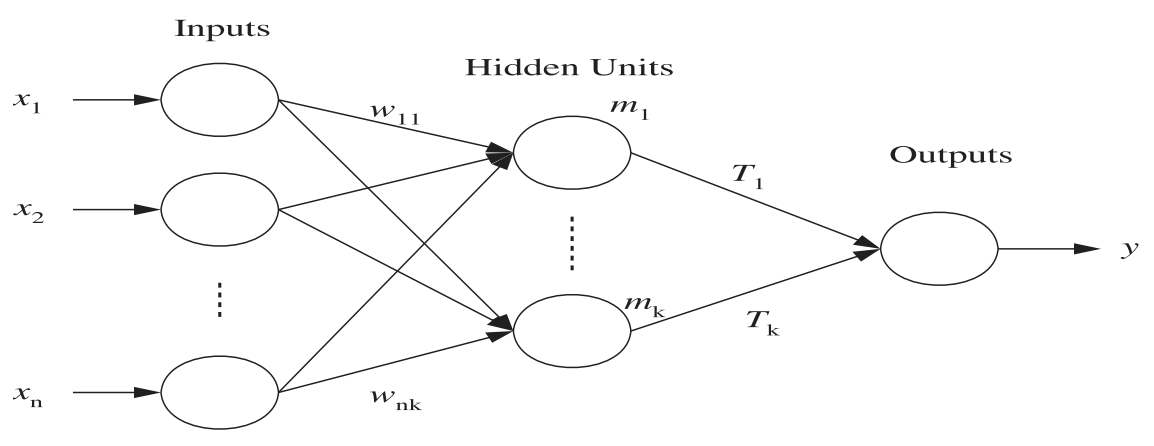
\includegraphics[width=\textwidth]{Chapter5/figures/feedforwardneuralnet}
	\caption{A three layer feed forward neural network.}
	\label{fig:mlp}
\end{figure}


\subsection{Support Vector Regression}

A support vector regression model maps input data, x, into a higher-dimensional feature space non-linearly. Given the input data\\ $(x_1,y_1), \ldots,(x_i,y_i),\ldots,(x_n,y_n)\allowbreak$ where $x_i$ are input patterns, and $y_i$ is the associated output value of $x_i$, the support vector regression solves an optimization problem \cite{Shu2006,Chen2004}

\begin{equation}
\min_{\omega,b,\xi,\xi^{*}}\frac{1}{2}\omega^T\omega+C\sum_{i=1}^{n}(\xi_i+\xi_i^*)
\end{equation}

subject to
\begin{align}
\begin{multlined}
\label{svr:constrains}
y_i-(\omega^T\phi(x_i)+b)\leq\varepsilon+\xi_i^{*},\\
(\omega^T\phi(x_i)+b)-y_i\leq\varepsilon+\xi_i,\\
\xi_i,\xi^*_i\geq0,i=1,\ldots,n
\end{multlined}
\end{align}


where $x_i$ is mapped to a higher dimensional space by the function $\phi$, $\xi$ and $\xi^*_i$ are slack variables representing the lower and upper training errors respectively subject to the $\varepsilon$-intensive tube $(\omega^T\phi(x_i)+b)-y_i\leq\varepsilon$. The constant $C>0$ determines the trade-off between the flatness and losses. The parameters which control regression quality are the cost of error $C$, the width of the tube $\varepsilon$, and the mapping function $\phi$ \cite{Shu2006,Chen2004}. 

The constraints of \eqref{svr:constrains} imply that we put most data $x_i$ in the tube $\varepsilon$. If $x_i$ is not in the tube, there is an error $\xi_i$ or $\xi_i^*$ that can be minimized in the objective function. Support vector machines avoid under-fitting and over-fitting of the training data by minimizing the training error $C\sum_{i=1}^n(\xi_i+\xi_i^*)$ as well as the regularization term $\frac{1}{2}\omega^T\omega$. Since $\phi$ might $x_i$ to a high or infinite dimensional space, instead of solving $\omega$ for \eqref{svr:constrains} in a high dimension, its dual problem is solved with \cite{Shu2006,Chen2004}

\begin{align}
\min_{\alpha\alpha^*}\frac{1}{2}(\alpha-\alpha^*)^TQ(\alpha-\alpha^*)+\varepsilon\sum^n_{i=1}(\alpha_i+\alpha_i^*)+\sum_{i=1}^ny_i(\alpha_i-\alpha_i^*)
\end{align}

subject to 
\begin{align}
\begin{multlined}
\sum_{i=1}^n(\alpha_i-\alpha_i^*)=0,\\
0\leq\alpha_i,\alpha^*_i\leq C,i=1,\ldots,n
\end{multlined}
\end{align}

where $Q_{ij}=\phi(x_i)^T\phi(x_j)$. However, this inner product may be expensive to compute because $\phi(x)$ has too many elements. Hence, we apply a "kernel trick" to do the mapping implicitly. That is, to employ some special forms, inner products in a higher space yet can be calculated in the original space \cite{Shu2006}. An example of the radial basis function kernel is listed below:
\begin{equation}
\phi(x_i)^T\phi(x_j)=e^{-\gamma\left|x_1-x_2\right|^2}
\end{equation}

\subsection{Random Forests}

Random forests are formed by an ensemble of tree-based models. They can be used either in regression or classification. The base model will be a regression tree for regression or classification tree for classification. 

At each split in a tree within the forest, the test is chosen from a randomly selected sub-set of the independent variables. Also, the trees are not pruned. Random forests can be used for feature and outlier detection \cite{Herrera2010}.




\subsection{Evaluation}

For the measure of prediction accuracy this paper adopts mean absolute percentage error (MAPE). The formula is as follows:

\begin{equation}
MAPE=\frac{1}{n}\sum_{i=1}^n\left|\frac{y_i-\hat{y}_i}{y_i}\right|\times 100\%
\end{equation}

where $y_t$ is the actual value, $\hat{y}_t$ is the forecast value and $n$ is the number of points forecast \cite{Li2016}.


\section{Methodology}

\subsection{Data Collection}

Smart meter data obtained from the Irish Social Science Data Archive (ISSDA) on the 28th of September 2017 was used in this study. The Commission for Energy Regulation released a public dataset of anonymised smart meter data from the "\textit{Electricity Smart Metering Customer Behaviour Trials}." This dataset is made up of over 5000 Irish homes and businesses and is sampled at 30 minute intervals.

The data was split into two partitions, the training set and the testing set. The training set made up the first 11 months of data and was used to parametrise the models, whereas the test set is made up of the remaining 6 months of data. The test set was used for evaluation of the models proposed.

Figure \ref{fig:single_user} demonstrates the electricity consumption profile of a single week for a single user. Whilst it can be seen that electricity usage changes significantly between days, a pattern of behaviour is exhibited. There is a large peak displayed each day in the evening, as well as a peak earlier during the day. It can therefore be assumed that this customer has a habitual behaviour pattern. 

Figure \ref{fig:multiple_users} shows eight different residential customer load profiles on the 22nd June. It can be seen that the daily load profile changes between each customer. The consumers use varying quantities of electricity and at different times. 


\begin{figure}
	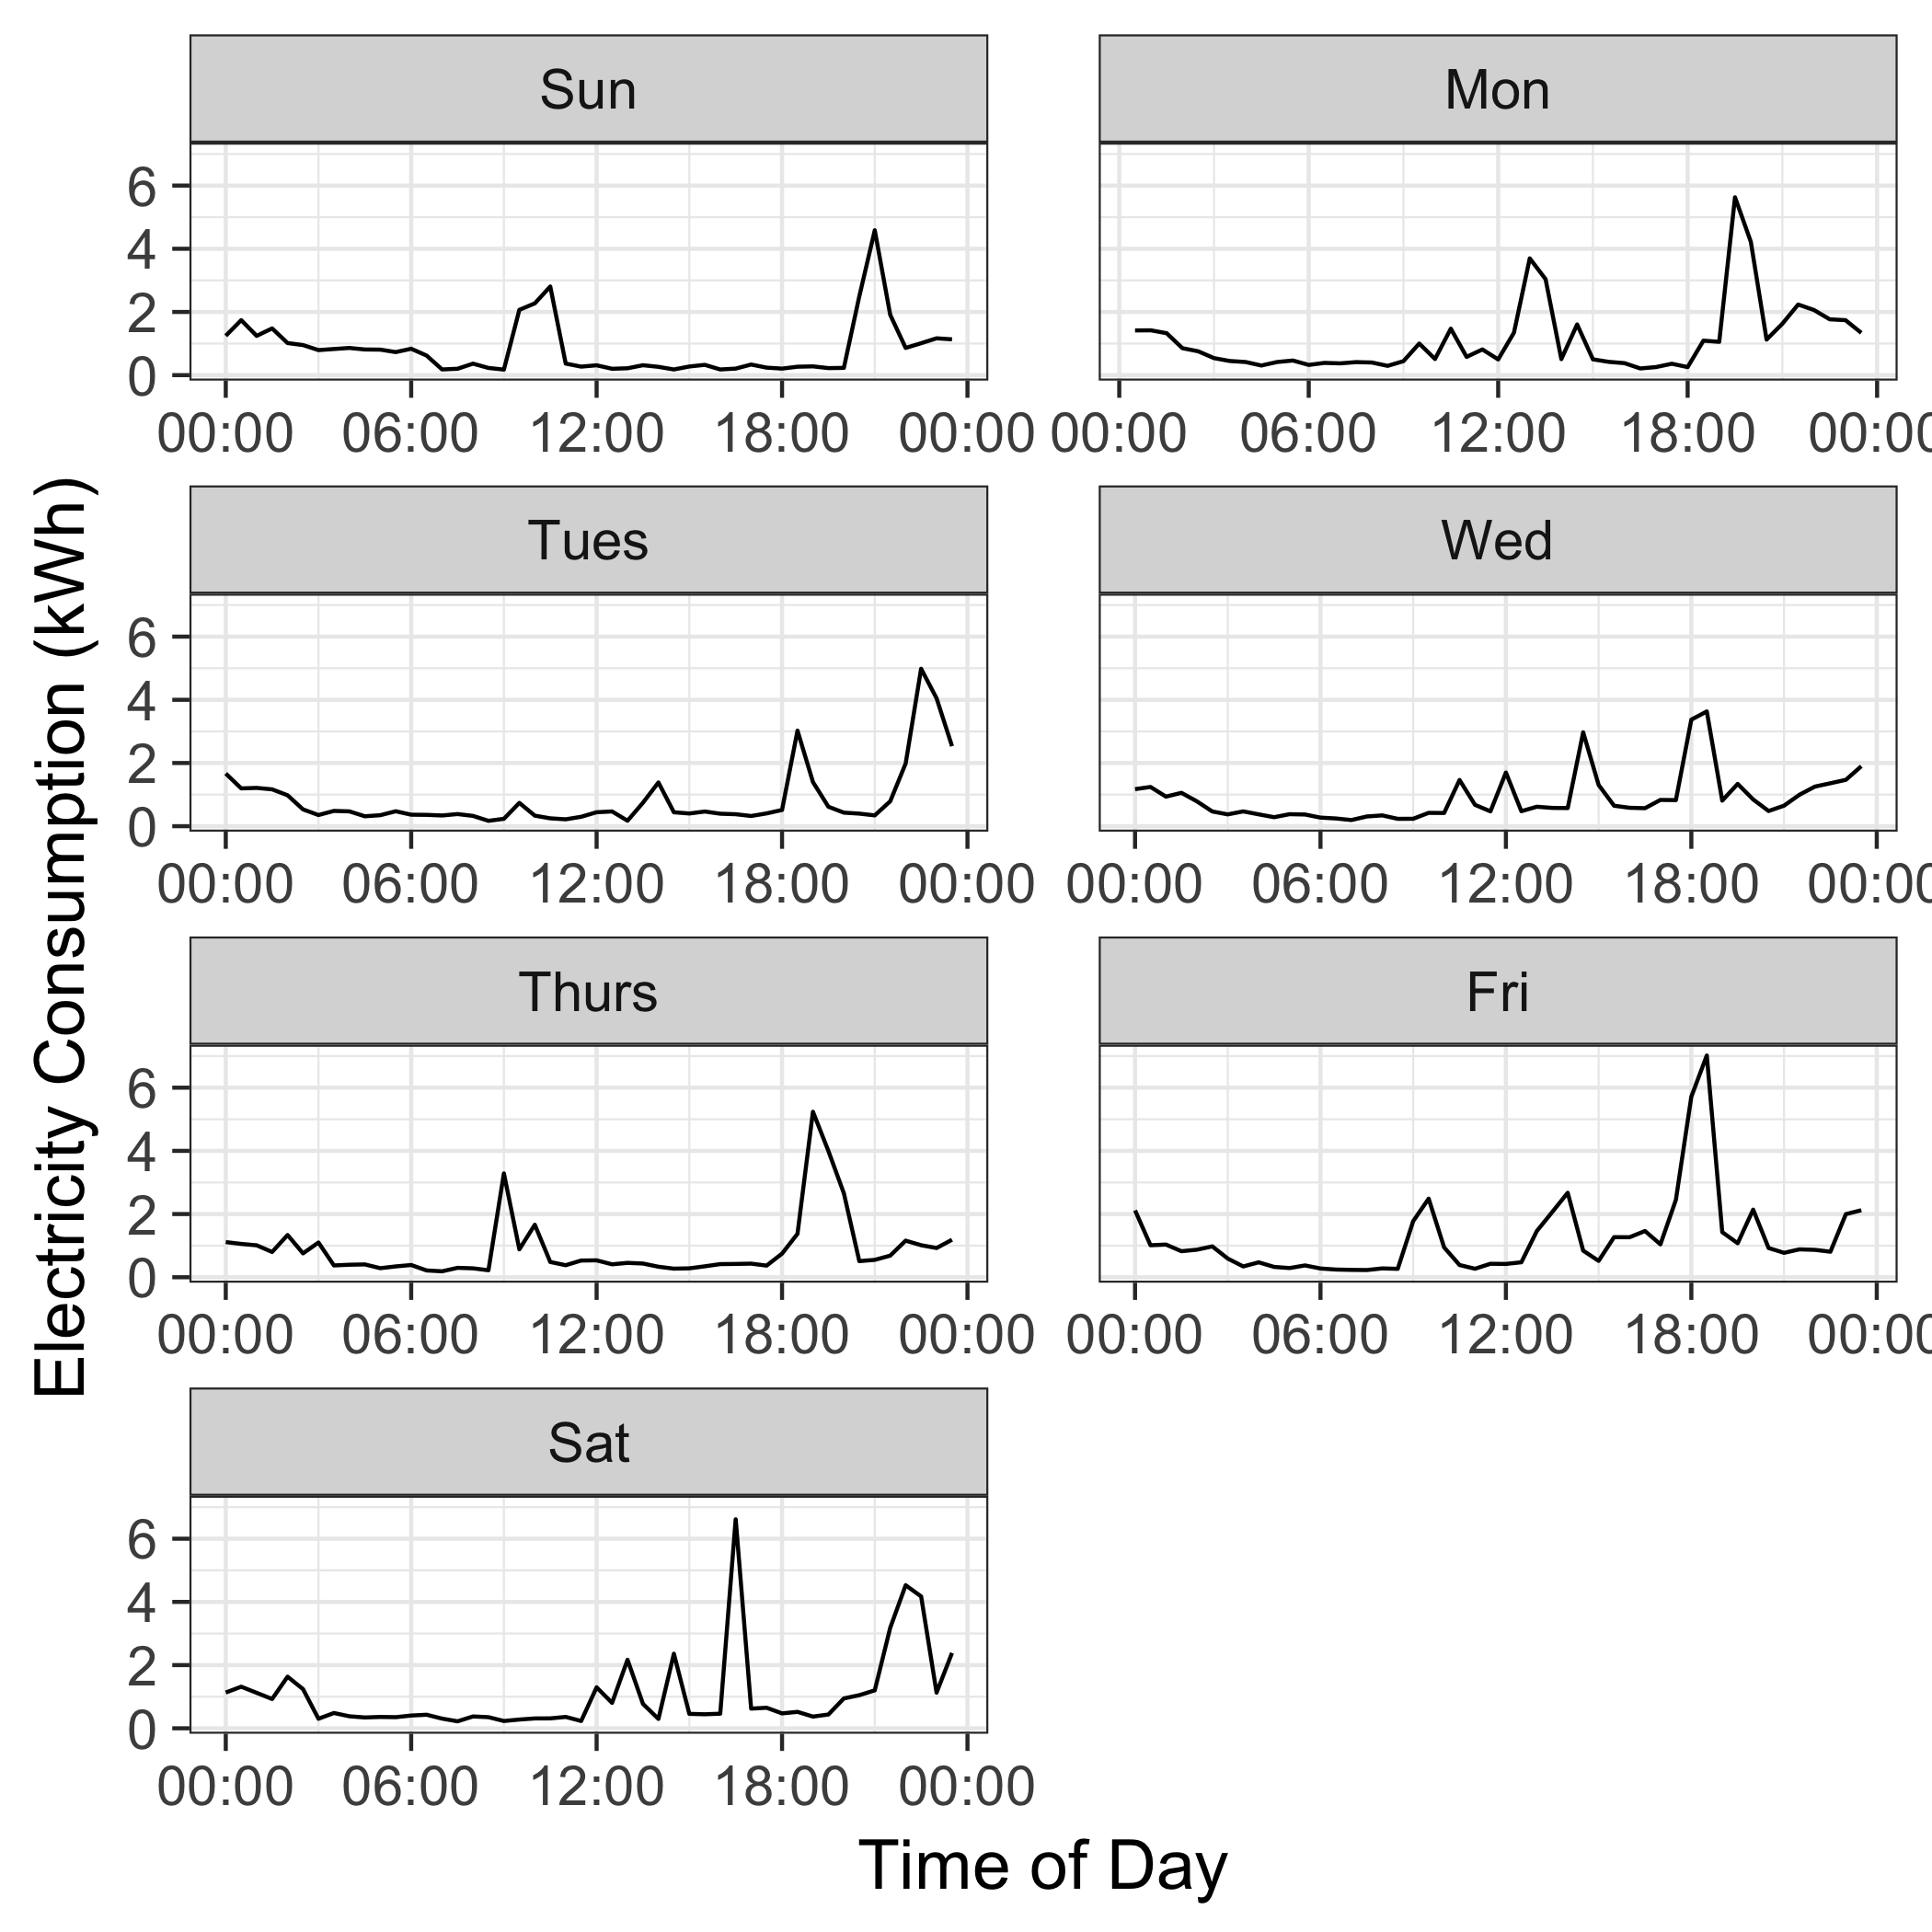
\includegraphics[width=0.76\textwidth]{Chapter5/figures/Rplot01}
	\caption{Daily load profiles for a single customer over a week between 20th July 2009 and 27th July 2009.}
	\label{fig:single_user}
\end{figure}

\begin{figure}
	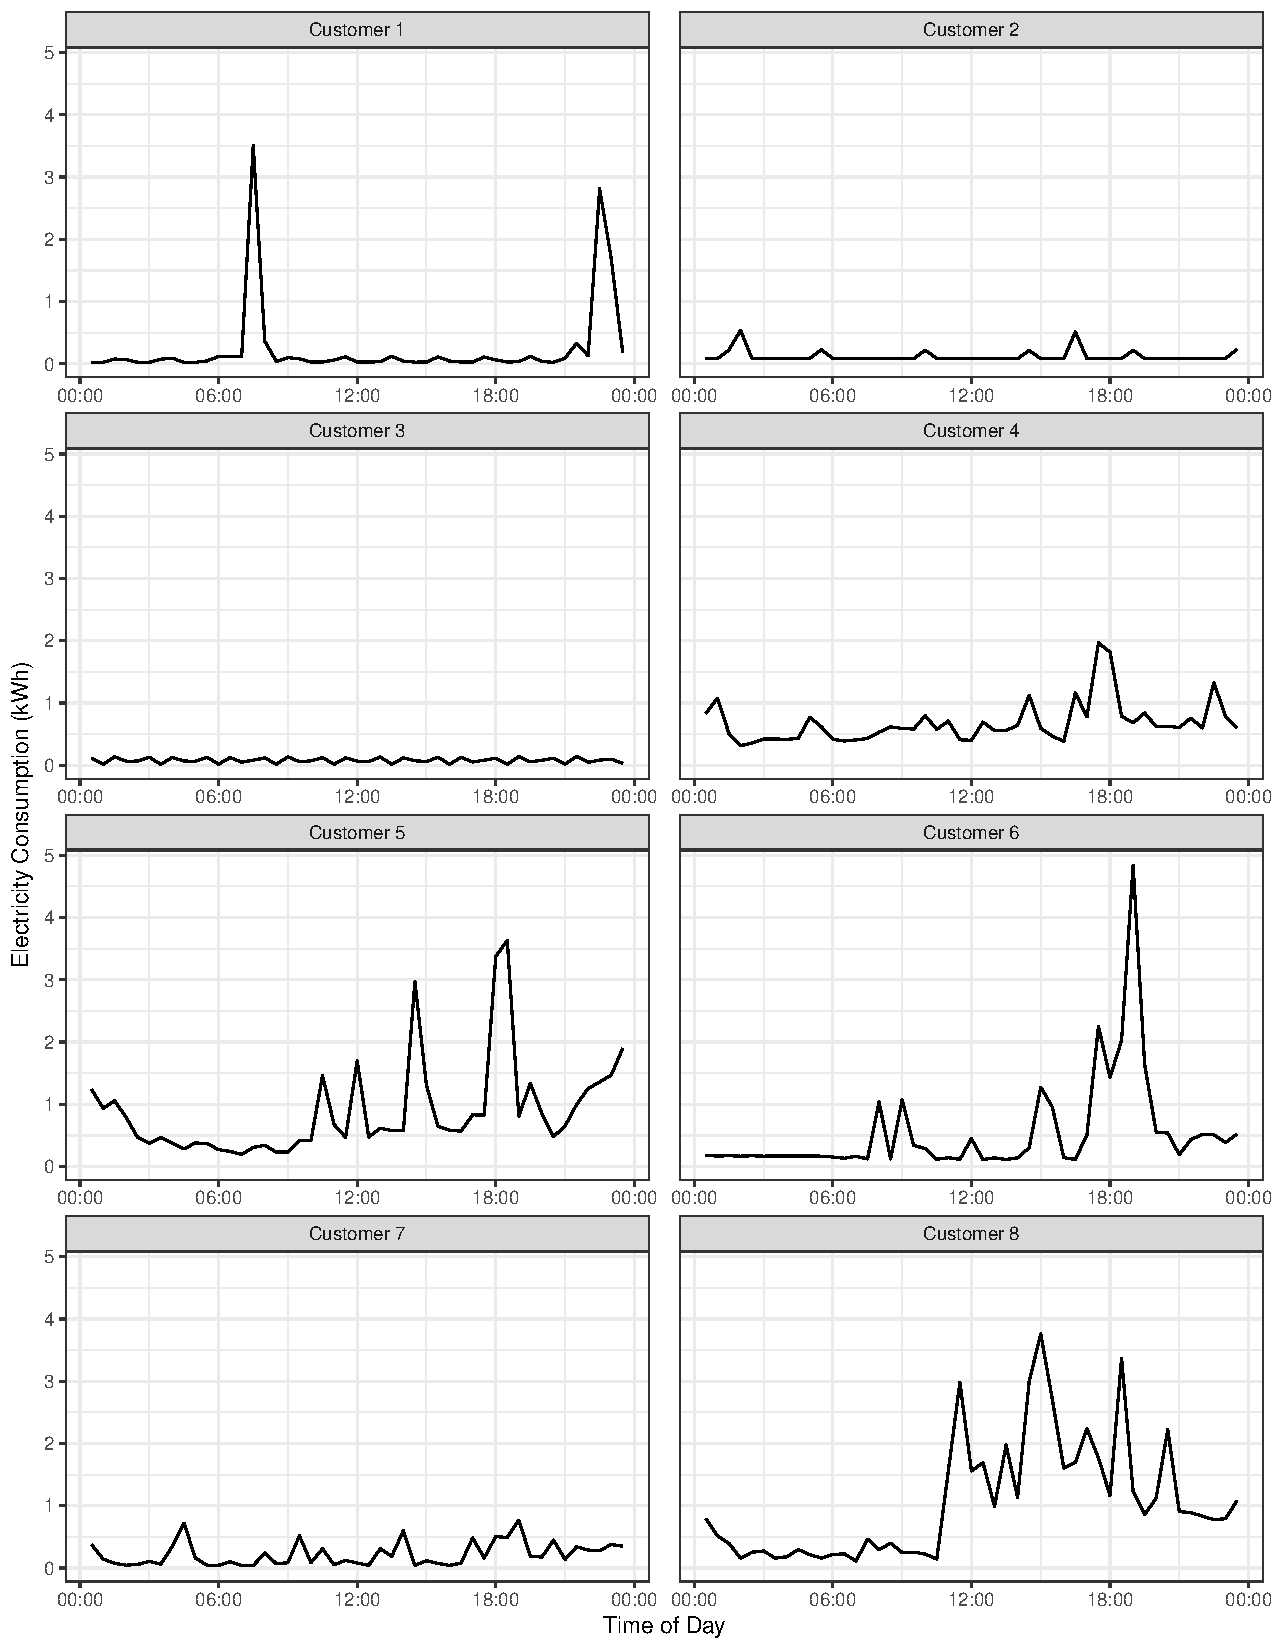
\includegraphics[width=0.76\textwidth]{Chapter5/figures/Rplot02}
	\caption{Daily load profiles for different customers over a single day on the 22nd June 2009.}
	\label{fig:multiple_users}
\end{figure}

It is clear from these figures that electricity consumption changes per person, per day. To capture this variability between customer types these customers are clustered and then aggregated. Each of the different aggregated electricity consumptions should provide a more a less stochastic load profile, and therefore increase the accuracy of the models.

\subsection{Clustering}

It is proposed that clustering similar customer load profiles and aggregating each cluster's electricity consumption will improve the accuracy of the models. 

To cluster the load profiles different options were considered. Hierarchical clustering using metrics such as euclidean and wavelet distance metrics were tried, as was \textit{k}-means.\textit{ K}-means proved to be the most robust and best performing clustering algorithm, and thus was chosen for use in this paper.


To select the optimum number of clusters (\textit{k}) cross-validation was implemented. This allowed us to compare the results for each of the models and select the \textit{k} which was most appropriate.

The cross-validation method proposed worked by trying a different number of clusters per algorithm, and testing for the resulting MAPE. The optimum number of clusters with a low MAPE is then chosen. In this paper we varied \textit{k} between 1 and 7. We fit multiple models per cluster and predicted the next 6 months electricity consumption.

With \textit{k}-means clustering it is possible that with the same initialization number of clusters, different clusters are formed. This is due to the algorithm converging to a local minima. To overcome a local minima the \textit{k}-means algorithm is run multiple times and the partition with the smallest squared error is chosen \cite{Jain2010}. In our case, the \textit{k}-means clustering algorithm is run 1000 times to avoid local minima. 

The clustering technique implemented in our paper used a scaled input approach. The daily load profile was averaged for each customer based on each day of the training data. The data was then scaled so that households of different sizes but with similar usage profiles were clustered together. This data, which is made up of a \textit{m-by-n} matrix, where \textit{m} is equal to the total number of meters and \textit{n} is equal to 48 (two readings for each hour in the day).


\subsection{Aggregating Demand}

Once each smart meter is assigned to a different cluster, the total electricity consumed per smart meter in each cluster is aggregated. This provides a partial system load. A different model is trained on each of the different partial system loads, and the resulting forecasts are then aggregated to generate the total system load forecast. The total system load forecast is then used to evaluate the accuracy of each of the different models using MAPE. 

Random Forests, Support Vector Regression, Multilayer Perceptron neural networks and Long-Short Term Memory neural networks were implemented, and a comparison between the different models were made. 

These models were chosen due to their ability to model multivariate non-linear relationships. They are data-driven methods and therefore suited to this type of problem.

\subsection{Feature Selection}

Each component of the training data is known as a feature. Features encode information from the data that may be useful in predicting electricity consumption. 

\subsubsection{Calendar Attributes}

Due to the periodicity of the electricity consumption daily, weekly and annually, the calendar attributes may be useful to model the problem. The calendar attributes included are as follows:

\begin{itemize}
	\item Hour of day
	\item Day of the month
	\item Day of the week
	\item Month
	\item Public holidays
\end{itemize}

With these attributes, the daily, weekly and annual periodicity can be taken into account.

It is noted that electricity consumption changes on a public holiday such as Christmas or New Years Eve. It is therefore proposed that public holidays in Ireland are input into the model as features to take these changes into account. 

\subsubsection{Time Series Data}

As well as the calendar attributes it is important to consider the historical load demand. This allows the time-series element to be taken into account by the models. 

To do this a lagged input of the previous 3 hours, the previous 3 hours of the previous day, and the previous 3 hours of the previous week were used. For example, to predict the electricity consumed on the 21st December 2010 at 12:00pm the electricity between 9:00pm and 11:30pm on the 21st of December are used as inputs, and the times between 9:00pm and 12:00pm on the 20th and 14th of December.

Long-Short Term Memory neural networks remember values over arbitrary time intervals. They can remember short term memory for a long period of time, for this reason 5 lagged inputs of the previous two and a half hours were used as features to the long-short term memory network.

\subsubsection{Data Representation}

Once useful information is selected we must encode the data for input into the models. To encode the day of the week seven binaries are utilised. Six of the binaries are for Monday through to Saturday. When all six binaries are equal to zero Sunday is encoded. A single binary for public holidays is included. Eleven binaries are used for month of the year, with the first eleven representing January to November, with December represented by all zeros in the calendar binaries. The current hour and date are input using a numerical attribute. The lagged data inputs, such as previous hour's electricity usage are also input using a numerical attribute for each entry, totalling 20 attributes (six half hourly entries for each 3 hour period multiplied by three days plus 2 entries for the time to be predicted on the previous day and week). Table \ref{tab:feature} displays these features.


\begin{table}
	\caption{List of Input Data for Models}
	\label{tab:feature}
	\begin{tabular}{p{3cm}p{3cm}p{8.5cm}}
		\toprule
		Input & Variable      & Detail description \\
		\midrule
		1     & Hour          & Single numeric input representing hour of the day                                                                                              \\
		2     & Day of month  & Single numeric input representing day of the month                                                                                             \\
		3-9   & Day of week   & Six binary digits representing calendar information regarding day of the week                                                                                            \\
		10-21 & Month         & Eleven binary digits representing calendar information regarding month                                                                                         \\
		22-42 & Lagged inputs & Twenty numeric inputs representing lagged inputs of previous 3 hours, previous 3 hours of previous day including hour to be predicted, and previous 3 hours of previous week including hour to be predicted \\
		43    & Holiday       & One binary digit representing whether the day was a public holiday  \\     \bottomrule                                                           
	\end{tabular}
\end{table}


\subsection{Implementation}

\subsubsection{Support Vector Regression}

To implement a support vector regression model a variety of parameters must be chosen. These parameters influence the performance of the model. To select these parameters cross-validation was implemented. The data was split 75\% into training data, and the remaining 25\% into test data.

To choose the optimum support vector machine kernel cross-validation was used, with 75\% acting as the training data and 25\% as the test. The kernels compared were polynomial, radial basis function (RBF) and the linear kernel.

The parameter values selected are shown in Table \ref{tab:kernel}. From the cross-validation the linear kernel was found to be the best performing. For this reason the linear kernel was utilised for prediction of electricity consumption in this paper.

\begin{table}
	\caption{Prediction Accuracy Based on Type of Kernel}
	\label{tab:kernel}
	\begin{tabular}{ccl}
		\toprule
		Kernel Type& Kernel Parameters & RMSE\\
		\midrule
		Linear & No values & 0.02102779\\
		RBF & C=2, $\gamma=0.016$ & 0.02444950\\
		Polynomial & C=2, $d=2, r=2$ & 0.03145719 \\
		\bottomrule
	\end{tabular}
\end{table}


\subsubsection{Random Forest}

To initialize the random forest algorithm with the number of variables randomly sampled as candidates at each split, cross-validation was used. Once again, 75\% of the data was used for training and the remaining 25\% for testing.

\begin{figure}
	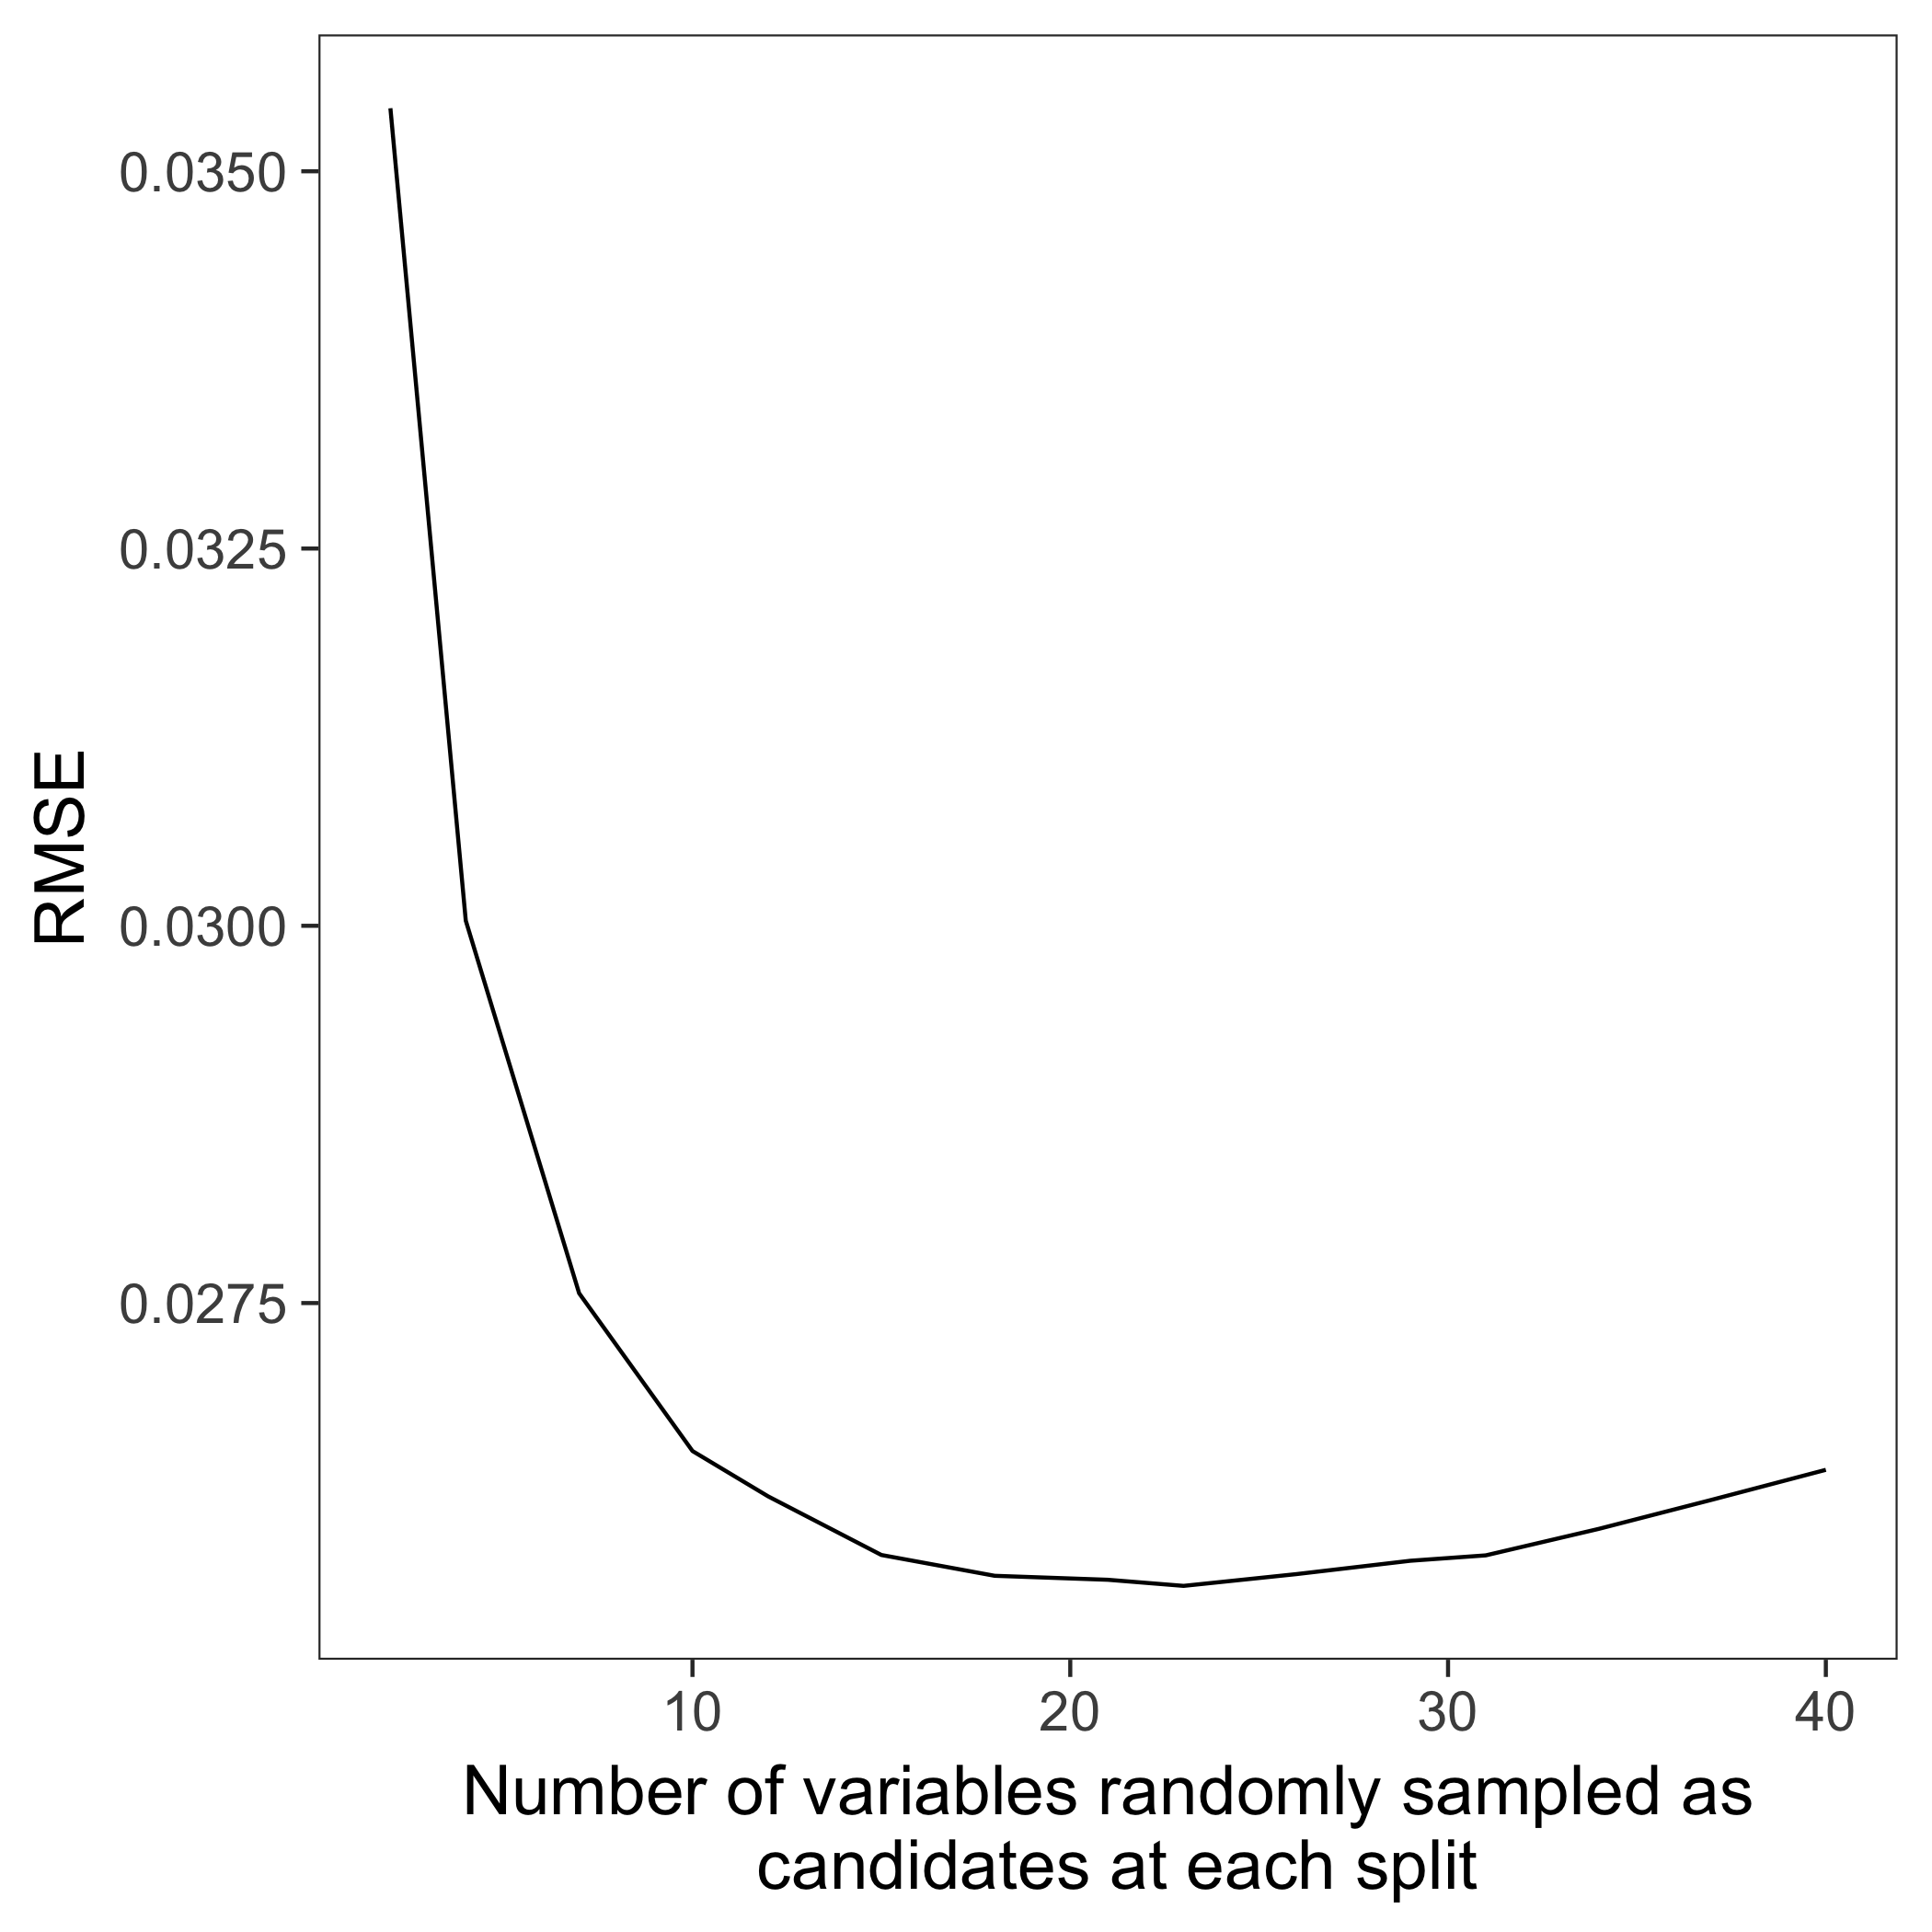
\includegraphics[width=0.5\textwidth]{Chapter5/figures/rforest_parameter_tuning}
	\caption{RMSE vs Number of variables randomly sampled as candidates at each split in the random forest model.}
	\label{fig:rf_param_tune}
\end{figure}


Figure \ref{fig:rf_param_tune} shows the results of tuning the parameter of number of variables randomly sampled as candidates at each split. The optimum number was found to be 23. Either side of this value the RMSE increases. Therefore the value 23 was selected to be the number of variables randomly sampled as candidates at each split in the random forest model


\subsubsection{Multilayer Perceptron}

A feed-forward multilayer perceptron is a common neural network architecture used for the prediction of time series data, which has comparable, and occasionally better than statistical models \cite{Hill1994}. 

The first step when designing a multilayer perceptron neural network is to design the architecture. For this case the number of input neurons is set to 41 (see table \ref{tab:feature}). Once an input for each neuron is entered, the output layer must be designed. Due to the fact that we are forecasting only one time step ahead (30 minutes ahead) one output neuron is required.

The next step is to design the architecture of the hidden layers. To accomplish this cross-validation is utilised as per the previous models. A maximum of 3 hidden layers were tested and the results analysed. A similar method to Fan \textit{et al.} was implemented to choose the number of neurons and hidden layers, a technique known as the Levenberg-Marquardt technique \cite{Fan2009}. The Levenberg-Marquardt is a technique suitable for training medium-sized artificial neural networks with a low mean-squared error. 

The fundamental rule is to select the minimum number of neurons in the hidden layer so as to capture the complexity of the model, but not too many as to introduce over-fitting, which results in a loss in generalization of the algorithm.

The method begins by choosing a small number of neurons and gradually increasing the number each time the model is trained and the forecast error obtained. The forecast error is monitored until an optimum value is found, to which no further improvement is noted. Once the optimum number of neurons in the layer is obtained an additional layer is added, and the same technique is used.

Using this technique an optimal architecture with three layers is obtained. The first layer contained two neurons, the second contained five, and the third contained four.



\subsubsection{LSTM}

To initialize the LSTM cross-validation was used to select the number of stacked layers and memory units. Similarly to the technique used for the multilayer perceptron, the Levenberg-Marquardt was used. The optimum number of layers was found to be 2, with a total of 50 memory units.



\section{Results}

To test the accuracy of the trained model the data was split into a training and test set. The data between the 14th of July 2009 and the 15th of June 2010 was used as the training data, whilst the data between the 15th of June 2010 and 31st of December 2010 was used for testing purposes. The test set is separate from the training set and not used during training. 

28 independent forecasting models are constructed for random forests, support vector regression, LSTM's and multilayer perceptron neural networks at each of the groups with $k$ varying from 1 to 7. This was done to determine the optimal number of clusters. We evaluated the MAPE of the overall prediction. 

Figure \ref{fig:results} displays the accuracy of the models trained at different numbers of clusters ($k$). 

The results show that introducing a cluster number larger than 1 does improve results in all cases. The optimum value for $k$ for random forests and support vector regression was found to be 4. After this the accuracy diminishes slightly.

The multilayer perceptron and LSTM neural network display a large increase in accuracy at 2 clusters. For the LSTM network 2 is the optimum number of clusters, whereas neural networks show a dramatic increase in accuracy at 5 clusters.

It can be seen from figure \ref{fig:results} that the best performing model is the random forest, followed by support vector regression. 

\begin{figure}
	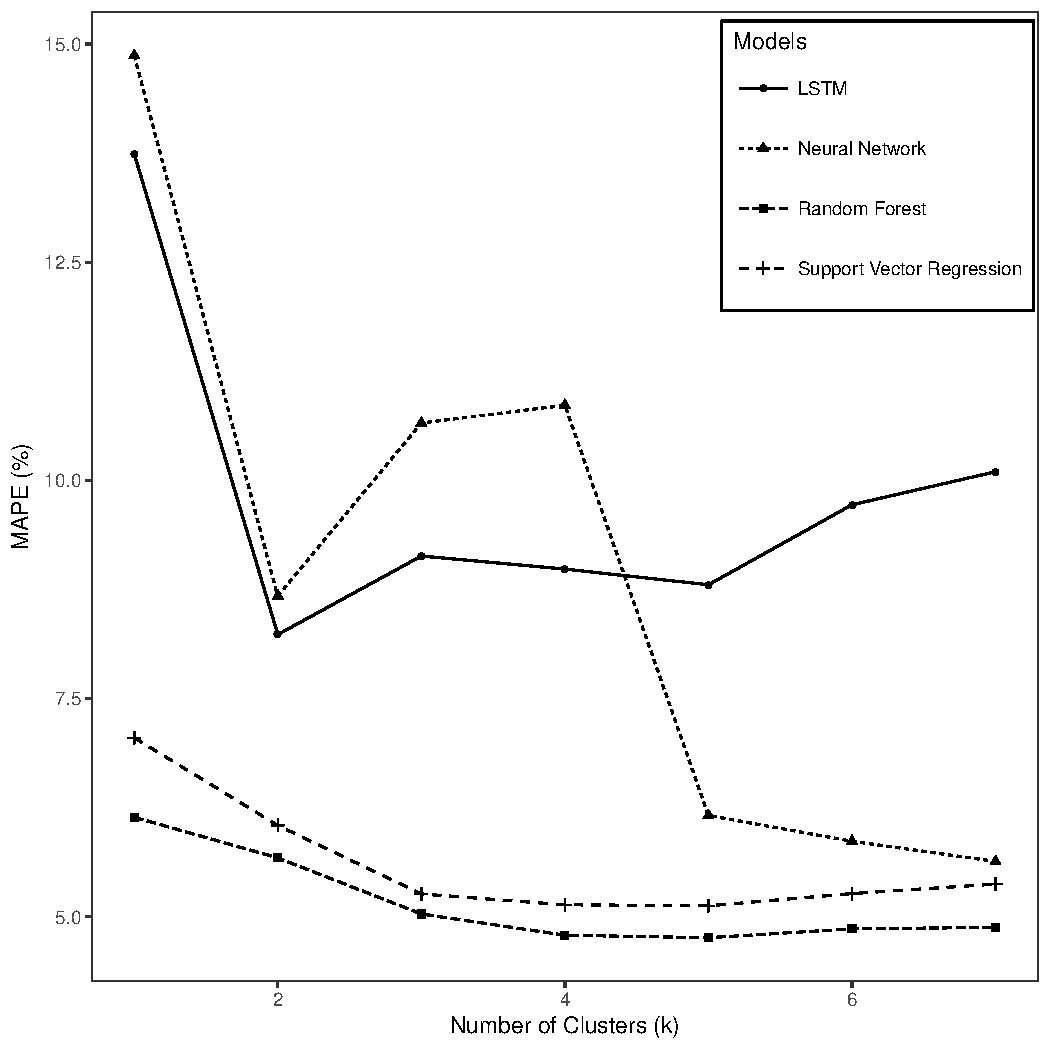
\includegraphics[width=0.7\textwidth]{Chapter5/figures/results.pdf}
	\caption{Comparison of accuracy of models forecasting electricity with varying number of clusters.}
	\label{fig:results}
\end{figure}

\begin{table}
	\caption{Lowest MAPE per model.}
	\label{tab:results_mape}
	\begin{tabular}{cc}
		\toprule
		Model& Highest Accuracy MAPE (\%) \\
		\midrule
		LSTM & 8.23 \\
		Neural Network & 5.63 \\
		Random Forest & 4.76  \\
		Support Vector Regression & 5.13  \\
		\bottomrule
	\end{tabular}
\end{table}

Table \ref{tab:results_mape} shows that the best performing model is a random forest with a MAPE of 4.76\%. 

\section{Conclusion}

The availability of high granularity data produced by the smart grid enables network operators to gain greater insights into their customer behaviour and electricity usage. This enables them to improve customer experience, utility operations and power management. We demonstrated that implementing the \textit{k}-means clustering algorithm to group similar customers improved the accuracy of every one of the different models tested. Distinct models were trained for each of the clusters and the individual forecasts aggregated for the total aggregated forecast. It was found that random forests outperformed  the other models at all levels of clustering, and that the optimum number of clusters was 4. Whilst the dataset used focused on residential data it is expected that applying a similar clustering technique on commercial properties would have a similar effect.

In future work we will look into the features that best aid in the forecasting of electricity consumption, try a wider variety of models in an ensemble manner and try different clustering techniques such as self-organizing maps (SOM) to obtain better accuracy measures. We will also compare different prediction error measures.


